\documentclass[a4paper, fontsize = 14pt]{article}
\usepackage{hyperref}
\usepackage[warn]{mathtext}
\usepackage[english,russian]{babel}
\usepackage[utf8x]{inputenc} 
 
%математика
\usepackage[mathscr]{eucal}
\usepackage{amsmath,amsfonts,amssymb,amsthm,mathtools}
\usepackage{icomma}
\usepackage{wasysym}
\usepackage{mathrsfs}
 
%оформление текста
\usepackage{setspace}
\onehalfspacing
\usepackage{indentfirst}
\usepackage{scrextend}
 
%геометрия
\usepackage{geometry}
\geometry{left=25mm,right=25mm,
 top=25mm,bottom=30mm}
 
%графика
\usepackage{wrapfig}
\usepackage{graphicx}
\usepackage{pgfplots}
\usepackage{tikz}
\RequirePackage{caption}
\DeclareCaptionLabelSeparator{defffis}{ --- }
\captionsetup{justification=centering,labelsep=defffis}
 
%таблицы
\usepackage{array,tabularx,tabulary,booktabs} 
\usepackage{longtable}  
\usepackage{multirow} 
 
%ссылки
\usepackage{hyperref}
\usepackage{xcolor}
\definecolor{grn}{HTML}{57A14F} %зеленый
\definecolor{rd}{HTML}{E53C44} %красный 
\definecolor{bl}{HTML}{282691} %синий 
\definecolor{bbl}{HTML}{001B6C} %темно-синий
\hypersetup{		
    colorlinks=true,       	
    linkcolor=bbl,          % внутренние ссылки
    citecolor=rd,          % на библиографию
    filecolor=magenta,      % на файлы
    urlcolor=bl           %внешние источники
}
 
% Колонтитулы
\usepackage{fancyhdr} 
 	\pagestyle{fancy}
 	\renewcommand{\headrulewidth}{0.15mm}  
 	\renewcommand{\footrulewidth}{0.15mm}
 	\lfoot{МФТИ, 2021}
 	\rfoot{\thepage}
 	\cfoot{}
 	\rhead{}
 	\chead{}
 	\lhead{}
 
 
\begin{document}

\begin{center} \textbf{
Лабораторная работа №2.3.1[Б] \\ Современные средства получения и измерения вакуума \\
Мещеряков Всеволод, Б02-001, 11.03.2021}
\end{center} 

\subsection*{Введение}

Изучаются принципы получения и измерения высокого вакуума в экспериментальном стенде на основе компактного высоковакуумного откачного поста Edwards серии EXPT, вакууметров Edwards и вакуумных компонентов типа ISO-KF.

\subsection*{Общие сведения}

Вакуумом в физике называется состояние газа, при котором характерная длина свободного пробега молекул в газе сравнима по порядку величины с характерным линейным размером сосуда, в котором содержится газ.

В технике же вакуумом называется состояние газа, давление которого меньше атмосферного. 

Разделяют три типа вакуума: $\textbf{низкий}$, когда средняя длина свободного пробега значительно меньше характерного линейного размера рассматриваемого объема; $\textbf{средний}$, когда средняя длина свободного пробега сравнима с характерным линейным размером рассматриваемого объема; $\textbf{высокий}$, когда средняя длина свободного пробега значительно больше характерного линейного размера.

\subsection*{Ход работы}

\subsubsection*{II. Определение откачиваемого объёма и измерение скорости откачки форвакуумным насосом }

Выровняем давление во всех частях установки. Для этого откроем краны МК1, МК2, МК3, МК4 и шибер ШЗ, после чего впустим в систему атмосферный воздух через КН. Затем закроем КН, шибер ШЗ, кран МК3, а краны МК1, МК2, МК4 оставим открытыми. На схеме (Рис.1) зеленым обозначены открытые пути, по которым может перемещаться газ, и красным закрытые.

\begin{figure}[hbt]\label{risII}
\center{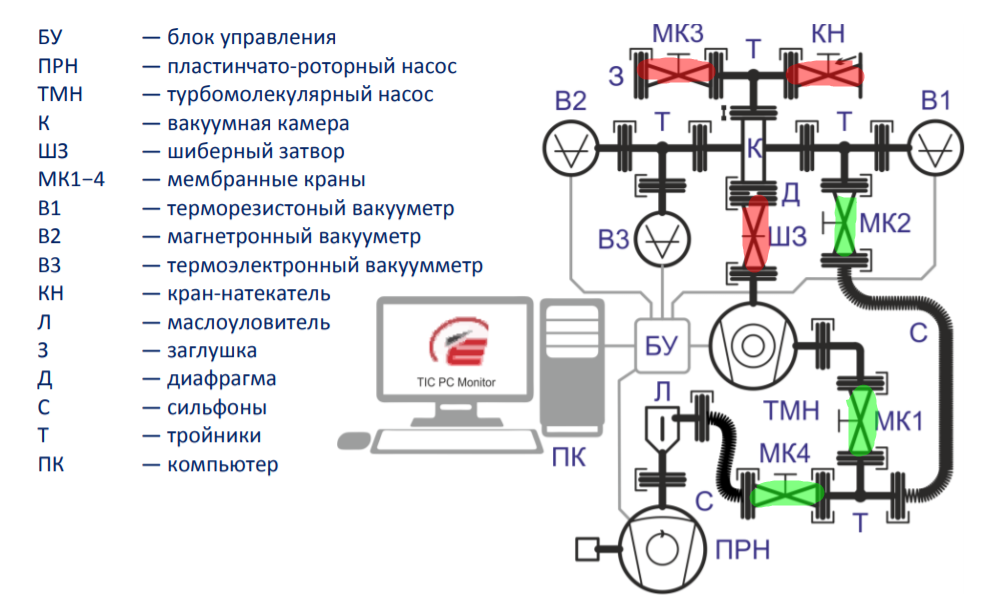
\includegraphics[scale=0.65]{lab231risII.png}}
\caption{\textit{Схема установки в исходном состоянии}}
\end{figure}

Запустим пластинчато-роторный насос с помощью компьютера и откачаем установку до предельного давления, которое определим по динамике показаний вакууметров. В какой-то момент их показания перестанут меняться, что будет соответствовать квазистатичной отчачке газа, попадающего в систему через щели. Зафиксируем время откачки и предельное давление в системе - таблица 1.

Отсоединим заглушку на МК3, после чего обезжирим вакуумные поверхности сильфона и трубок. Установим заглушку на другой конец сильфона и подключим его к МК3. При этом в сильфоне, согласно его паспорту, будет содержаться 252 мл воздуха. 

Остановим откачку воздуха из камеры К, закрыв МК2. Откроем МК3, чем дадим воздуху из сильфона заполнить вакуумную камеру К. Зафиксируем установившееся давление по показаниям вакууометра В1 - $P_{1}$ (давление в сильфоне и камере) в таблице 1. 

Выровняем давление в вакуумной камере и форвакуумной магистрали, закрыв МК1 и МК4, и открыв МК2. Зафиксируем установившееся давление по показаниям вакууометра В1 - $P_{2}$ (давление в камере, сильфоне и магистрали) в таблице 1. 

Откроем МК1, запустив воздух в объем турбомолекулярного насоса. Зафиксируем установившееся давление по показаниям вакууометра В1 - $P_{3}$ (давление в камере, сильфоне, магистрали и насосе) в таблице 1. 

Выключим пластиночно-роторный насос и откроем МК4, чем начнем подготовку установки к повторному измерению.  

Как видно из таблицы 1, приемлемая повторяемость была достигнута тремя измерениями. Из нее же с помощью закона Бойля-Мариотта вычислим полный объем установки $V_{уст}$, камеры К $V_{к}$, форвакуумной магистрали $V_{маг}$ и турбомолекулярного насоса $V_{тмн}$. Погрешности оценим, воспользовавшись паспортом вакууметра В1, ошибка которого влияет сильнее других факторов ($\approx~15\%$):
\[ V_{уст} = (914\pm64)мл,\, V_{к} = (712\pm51) мл, \, V_{маг} = (201\pm14) мл , \, V_{тмн} = (713\pm49) мл . \]

\begin{table}[htb]
\centering
\caption{Измерение объемов и времени откачки}
\begin{tabular}{|c|c|c|c|c|c|c|}
\hline
\textbf{\begin{tabular}[c]{@{}c@{}}номер   измерения \\      \textbackslash\\      величина\end{tabular}} & \textbf{1} & \textbf{$\sigma_{абс}$} & \textbf{2} & \textbf{$\sigma_{абс}$} & \textbf{3} & \textbf{$\sigma_{абс}$} \\ \hline
\textbf{$t_{откачка}$, с}                                                                                 & 157        & 0,5                     & 152        & 0,5                     & 157        & 0,5                     \\ \hline
\textbf{$P_1$, $\cdot 10^{2}$ мбар}                                                                       & 2,56       & 0,38                    & 2,63       & 0,40                    & 2,64       & 0,40                    \\ \hline
\textbf{$P_2$, $\cdot 10^{2}$ мбар}                                                                       & 2,14       & 0,32                    & 2,15       & 0,32                    & 2,18       & 0,33                    \\ \hline
\textbf{$P_3$, $\cdot 10^{2}$ мбар}                                                                       & 1,32       & 0,20                    & 1,32       & 0,20                    & 1,38       & 0,21                    \\ \hline
\textbf{$V_{уст}$, мл}                                                                                    & 922        & 64,54                   & 920        & 64,4                    & 901        & 63,07                   \\ \hline
\textbf{$V_{к}$, мл}                                                                                      & 731        & 51,17                   & 704        & 49,28                   & 703        & 49,21                   \\ \hline
\textbf{$V_{маг}$, мл}                                                                                    & 191        & 13,37                   & 216        & 15,12                   & 198        & 13,86                   \\ \hline
\textbf{$V_{тмн}$, мл}                                                                                    & 730        & 51,1                    & 741        & 51,87                   & 669        & 46,83                   \\ \hline
\end{tabular}
\end{table}
Из таблицы, которую компьютер заполнял в течение выполнения работы, возьмем данные зависимости давления в камере К от времени откачки пластинчато-роторным насосом. По зависимости $ln{P}$ от $t$ определим постоянную времени откачки $\tau$ в диапазоне давлений $10^0-10^{-2}$ мбар. Зная объем камеры К $V_{к}$, рассчитаем эффективную скорость ее откачки.

\begin{equation}
-\ln{(\frac{P(t)}{P_0})}=\frac{S}{V_к} t, \, \, k = \frac{S}{V_к} \, (c^{-1}).
\end{equation}

\[ k_1 = (21\pm4)\cdot10^{-2} \, (c^{-1}), \, k_2 = (19\pm4)\cdot10^{-2} \, (c^{-1}), \, k_3 = (19\pm3)\cdot10^{-2} \, (c^{-1}) \,. \]

Тогда из каждого $k_i$ получаем $S_i$, из которых за $S$ истинное берем наилучшее их значение. Эффективная скорость откачки форвакуумным насосом (ПРН) E2M1.5 : 
\[ S_{прн} \approx (138\pm23) \, (мл/с). \]


\subsubsection*{III Измерение скорости откачки турбомолекулярным насосом и определение предельного вакуума}

Отсоединим сильфон от установки, установим на его место заглушку. Откроем МК3 и с помощью ПРН избавимся от воздуха, который оказался запертым между заглушкой и краном. 

Откроем шибер ШЗ, закроем МК2, чем подготовим установку к откачке турбомолекулярным насосом. На рисунке 2 аналогично рисунку 1 отмечены открытые и закрытые краны:

\begin{figure}[hbt]\label{risIII}
\center{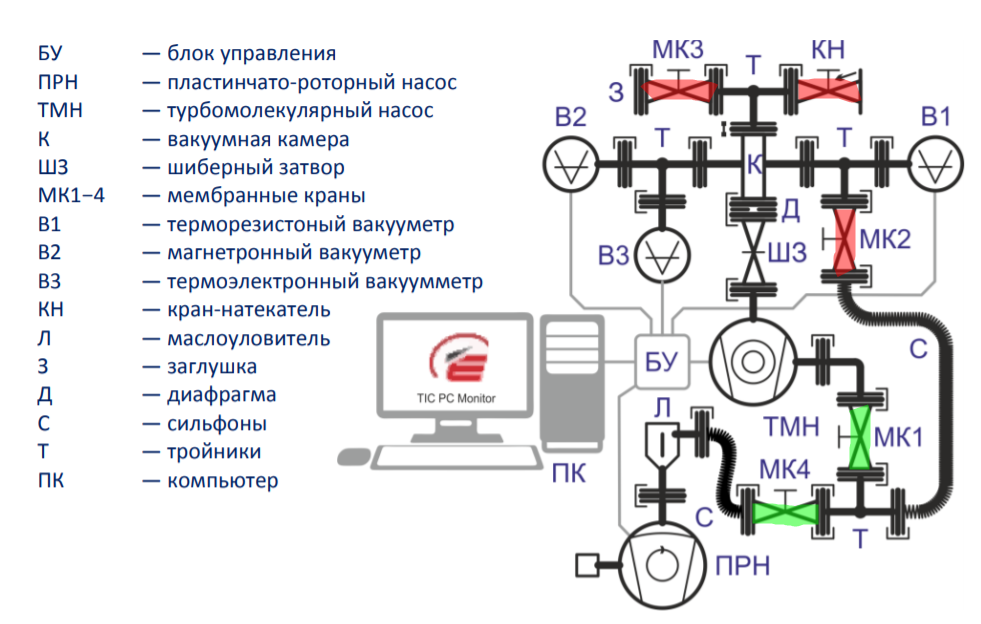
\includegraphics[scale=0.65]{lab231risIII.png}}
\caption{\textit{Схема установки в исходном состоянии}}
\end{figure}

Как видно из схемы, откачка будет производиться только из вакуумной камеры К ($V_{к} = (712\pm51)мл$). Проведем откачку турбомолекулярным насосом, определим которую по динамике вакууметров В2 и В3. Сравним данные, выводимые В1 и В2, В3, откуда увидим, что В1 прекратил работу еще на $10^{-4}$ мбар, когда В2 и В3 показывают $10^{-5}$ мбар.

Аналогично предыдущему пункту замерим время при котором давление в объеме проходит интервал в $10^{-5}-10^{-3}$ мбар. Зависимость также является экспоненциальной, поэтому линеанализируем ее для поиска константы. По МНК вычисляем коэффициент k и из формулы (1) с учетом обрабатываемого объема $V_{к}$ получаем величину эффективной скорости откачки турбомолекулярным насосом. Итоговая погрешность в наибольшей степени такова из-за погрешности вакууметров В2($\approx 30\%$) и В3($\approx 15\%$):
\[ S_{тмн} \approx (70\pm8)(мл/c). \]

Оценим натекание:

\[ Q_{н} = V_к \frac{(P_к-P_0)}{\delta t} = 3,6\cdot10^{-6} (\frac{кг\cdot м^2}{с}). \]

То есть за одну секунду в систему через один квадратный метр поступает примерно $4\cdot10^{-6}$ килограмм вещества. В нашем случае это воздух, поэтому можем оценить его количество $\approx 0,1 \, ммоль$. 

Оценим число Кнудсена для предельных давлений при откачке с помощью ТМН и ПРН. За характерный линейный размер возьмем 10 см, а средние длины свободного пробега при предельных давлениях посчитаем как:

\[ \lambda_{прн}=\frac{kT}{\sqrt{2}\pi d^2 p}\approx 2\cdot10^{-6} (м); \\
\lambda_{тмн}=\frac{kT}{\sqrt{2}\pi d^2 p}\approx 9\cdot10^{-5}(м).\]

Видно, что средние длины свободного пробега много меньше характерного линейного размера объемов, что соответствует высокому вакууму.

\subsection*{Вывод}

Эта работа позволила освоить основную технику откачки объемов до, как было выяснено, высокого вакуума. Были оценены эффективные скорости откачки двух разных типов насосов. Из результатов видно, что они оба имеют как достоинства, так и недостатки: ПРН работает в два раза быстрее ТМН, но его предельное давление меньше на три порядка. Была оценена величина течей, которая оказывается приемлемой в этой работе. Также были измерены рабочие объемы установки:
\[ V_{уст} = (914\pm64)мл,\, V_{к} = (712\pm51) мл, \, V_{маг} = (201\pm14) мл , \, V_{тмн} = (713\pm49) мл . \]

\end{document}